\documentclass[authoryear, 12pt, 5p, times]{elsarticle}
\usepackage{natbib} 
\usepackage{url}

\begin{document}
\begin{frontmatter}
\title{Creating updated, scientifically-calibrated mosaic images for the RC3 Catalogue}

\author[ucb]{Jung Lin Lee}
\ead{dorislee@berkeley.edu}
\author[ui]{Robert J. Brunner\corref{cor1}}
\ead{bigdog@illinois.edu}
\cortext[cor1]{Principal Corresponding author}
\address[ucb]{Astronomy Department, University of California at Berkeley, Berkeley, CA 94720-3411} 
\address[ui]{Department of Astronomy, University of Illinois, Urbana, IL 61801}

\begin{abstract}
The Third Reference Catalogue of Bright Galaxies (RC3) is a reasonably complete listing of 23,011 nearby, large, bright galaxies. By using the final imaging data release from the Sloan Digital Sky Survey, we generate scientifically-calibrated FITS mosaics by using the montage program for all SDSS imaging bands for all RC3 galaxies that lie within the survey footprint. We further combine the SDSS $g$, $r$, and $i$ band FITS mosaics for these galaxies to create color-composite images by using the STIFF program. We generalized this software framework to make FITS mosaics and color-composite images for an arbitrary catalog and imaging data set. Due to positional inaccuracies inherent in the RC3 catalog, we employ a recursive algorithm in our mosaicking pipeline that first determines the correct location for each galaxy, and subsequently applies the mosaicking procedure.
As an additional test of this new software pipeline and to obtain mosaic images of a larger sample of RC3 galaxies, we also applied this pipeline to  photographic data taken by the Second Palomar Observatory Sky Survey with $B_J$, $R_F$, and $I_N$ plates. We publicly release all generated data, accessible via a web search form, and the software pipeline to enable others to make  galaxy mosaics by using other catalogs or surveys.
\end{abstract}

\begin{keyword}
Image mosaics \sep RC3 catalog \sep Sloan Digital Sky Survey \sep Digitized Sky Survey \sep Montage \sep SExtractor
\end{keyword}

\end{frontmatter}

\section{Introduction}

Astronomers have a long history of cataloguing objects for subsequent study, for example the Messier catalog~\citep{messcat} and the New general Catalog~\citep[NGC;][]{ngccat} have provided valuable guidance to help astronomers study objects with similar properties. Today, we have entered the era of big data where large surveys such as the Sloan Digital Sky Survey~\citep[SDSS;][]{sdsstech} have uniformly surveyed large fractions of the entire sky, providing detailed photometric and astrometric information for millions of sources. However, the software pipelines that  process these valuable data are optimized for the more numerous small sources. As a result, large, nearby, and bright galaxies are essentially treated as contaminants. Yet these galaxies remain incredibly important, providing detailed insight into the dynamics of galaxies,
 as well as a low redshift sample with which to compare higher redshift galaxies. 

One of the more popular catalogs of nearby galaxies is the Third Reference Catalog of Bright Galaxies~\citep[RC3;][]{rc31991}, which is a catalog containing 23,011 galaxies with an apparent diameter greater than one arcminute at the $D_{25}$ isophotal level, with a total $B$-band magnitudes brighter than $~15.5$, and with a redshift not in excess of 15,000 km/s. The overall catalog is supplemented by selected galaxies that may only meet one or two of these conditions as well as some  nearby compact galaxies. Given the efficacy of this catalog, previous authors have used this sample as the basis for making image mosaics for a large sample of galaxies. 

The first such effort was made by~\cite{hbrc3}, who made color-composite images of select RC3 galaxies by using the SDSS $g$, $r$, and $i$ band images from the sixth SDSS data release. A subsequent effort by \citet{efigi}, dedicated to the study of galaxy morphology, generated a set of 4,458 FITS and color images by using the SDSS DR4 data. This latter effort employed a visual inspection to remove artifacts and galaxies with missing data. Finally, a separate effort, known as the NASA-Sloan Atlas\footnote{\url{http://www.nsatlas.org}}, has been undertaken to construct and analyze a complete set of galaxies within approximately 200 Megaparsecs~\citep{nsa}, which is the approximate redshift limit of the RC3 catalog.

Given the SDSS project has published their last imaging data release~\citep[DR10; ][]{dr10}, which includes the final photometric and astrometric calibrations, we have decided to update these previous efforts to make full, scientifically-calibrated image mosaics as well as color-composite images for all RC3 galaxies that lie within the SDSS DR10 footprint. As part of this process, we also generate updated coordinate positions for those galaxies with inaccurate catalog coordinates. We further generalize this software framework to produce scientifically calibrated FITS and color-composite images from any sky survey with astrometrically-calibrated FITS image data for an arbitrary galaxy catalog. We test this new pipeline by also constructing FITS image mosaics and color-composite images for all RC3 galaxies that lie within the Second Palomar Observatory Sky Survey~\citep[POSS-II;][]{poss2}. Our pipeline can be easily applied to existing data such as the Two Micron All Sky Survey~\citep[2MASS;][]{2mass}, or to future surveys such as the Dark Energy Survey~\citep[DES;][]{des} or the Large Synoptic Survey Telescope~\citep[LSST;][]{lsst}.

In Section~\ref{data-sec}, we introduce the RC3 catalog and the SDSS and POSS-II data that we use to generate mosaic images. Section~\ref{mosaic-sec} introduces our software pipeline and the relevant algorithmic details that enable us to obtain improved astrometric precision for the catalog galaxies. We discuss the actual construction of the image mosaics for the SDSS and POSS-II data in Section~\ref{results-sec}, before concluding the paper and discussing the overall project in Section~\ref{conc-sec}. 

\section{Data\label{data-sec}}

To construct large, calibrated image mosaics, we need two types of data. First, we need a catalog of galaxies; and second, we need an image data set. A number of different candidate galaxy catalogs exist; we also could follow the example used to develop the NASA-Sloan Atlas and construct a new catalog based on specific physical criteria. We choose, however, to use the RC3 catalog of galaxies~\citep{rc3}, which we detail in \S~\ref{sec:rc3}. For our imaging data, we actually selected two different surveys: the SDSS and the POSS-II. The SDSS uniformly surveyed a large fraction of the sky with digital detectors, while the POSS-II is an older photographic plate survey that covers nearly the entire sky. We discuss these two imaging surveys in detail at the end of this section. While not directly discussed in this paper, our pipeline approach could easily be extended to other datasets, such as the Two Micron Sky Survey~\citep{2mass}, the Wide-field Infrared Survey Explorer~\citep{wise}, and the Galaxy Evolution Explorer~\citep{galex}.

\subsection{The RC3 Catalog\label{sec:rc3}}

The simplest approach to constructing a uniform galaxy catalog is to  define a sample by limiting apparent brightness within a survey. Original attempts to accomplish this task date back to the original Harvard Survey of External Galaxies~\citep{shapley-ames}, which contained 1,249 objects brighter than 13$^{th}$ magnitude. Many of these galaxies were subsequently included in the University of Texas monographs in astronomy, which were predecessors to the RC3 catalog. The actual RC3 Catalog is an update to the Original and Second Reference Catalog of Bright Galaxies~\citep{rc2}. The original RC3 galaxy catalog compiled by \citet{rc3}, contains a  complete listing of 23,011 galaxies with $D_{25}$ apparent major isophotal diameter greater than one arcminute and with a total B-band magnitude greater than 15.5$^{th}$ magnitude. 

As the imaging data used to update these galaxies  came from various different imaging programs, the final, updated catalog is heterogeneous with a non-uniform distribution of updated galaxies. An update was published a few years after the original RC3 catalog by~\citet{rc3-94}. In this project, we use the RC3 catalogue information available through the VizieR Service\footnote{\url{http://vizier.u-strasbg.fr/viz-bin/VizieR?-source=VII/155}},  which contains the updated RC3 data published in 1994. After the RC3 catalogue was published, it was incrementally updated with new, published observations and subsequently maintained by Harold G. Corwin\footnote{\url{http://haroldcorwin.net/rc3/bugs.rc3}}. 

Since the RC3 catalog  is a reasonably complete representation of large, bright nearby galaxies in the extragalactic sky, it remains a popular catalog. Selected galaxies or complete subsets have been used in astrophysical studies of quasars and X-ray sources~\citep[e.g.,][]{walton-rc3}, and for galaxy morphology and clustering studies~\citep[e.g.,][]{best-rc3, knapen-rc3}.  The RC3 catalog also serves as a basis for statistical studies  in cosmology, for example within the New York University-Value Added Galaxy Catalog~\citep{nyuvagc}.

\subsubsection{Updating the RC3 Astrometry\label{sec:position}}

As described in \S\ref{mosaic-sec}, we use the montage toolkit to reproject and mosaic individual survey FITS images. Initially when we followed the standard mosaicking steps in montage, we obtained many mosaics with off-centered or missing RC3 galaxies. After further review, we realized that this effect was due to the inherent positional inaccuracy in the catalog, which, given the size of a typical RC3 galaxy, was surprising. On further reflection, however, this effect can be understood by the heterogeneous origin and updating of the RC3 catalog.

The entries in the RC3 catalog hosted by VizieR are astrometrically tied to the B2000.0 FK4 reference system. Due to the heterogenous positional updates, the RC3 galaxies are denoted with two different levels of accuracy: HH MM SS.s, DD MM SS for positions that have been updated  to an accuracy of approximately $5$--$8$ arcseconds, and  HH MM.m, DD MM for galaxies whose positional accuracy remains at approximately $1$--$2$ arcminutes as presented in the original catalog. The 1991 version of the RC3 catalog~\citep{rc31991} contains 5,492  galaxies that fall in the latter group. As a result, we developed an iterative mosaicking step within our pipeline, as discussed in~\S\ref{pos-sec}, to compute updated astrometric coordinates for those galaxies with poor astrometry so that we would have the target galaxy centered on the final mosaic.

\begin{table}
\footnotesize
    \begin{tabular}{llll}
    \hline
    ~                           & SDSS    & POSS-II             \\ \hline
    Imaging bands               & u, g, r, i, z  & $R_F$, $B_J$, $I_N$             \\
    Sky Coverage (\%)                & 35.28 & 78.27             \\
    Resolution ($^{\prime\prime}$/pix) & 0.396  & 1.7                 \\
    Imaging Technique           & CCDs    & Photographic Plates\\ \hline
    \end{tabular}
    \label{table:comptbl}
    \caption{{\footnotesize A summary of the two surveys processed in this work.}}
\end{table}

\subsection{SDSS}
The SDSS image data is acquired from the $2.5$-m telescope~\citep{sdss-tel} at the Apache Point Observatory in New Mexico. For our mosaics, we use the imaging data from the SDSS Data Release 10. The SDSS imaging camera~\citep{sdss-camera} was one of the first, large imaging cameras that leveraged Charge Coupled Devices (CCDs) as photon recording instruments. CCD detectors have obvious throughput advantages over photographic plates and also provide a near-linear response to input signals. In addition, the pixel resolution and mean seeing at Apache Point combined to provide a reasonable angular resolution, especially for large, bright galaxies. 

The SDSS imaging data is processed by the $\texttt{photo}$ pipeline~\citep{sdss-photo}, which is responsible for a number of different image processing procedures, including source detection, deblending, model-fitting, and astrometric and photometric calibration. We quantify the imaging quality of the SDSS data we use by the $\texttt{clean}$ flag\footnote{\url{http://skyserver.sdss3.org/dr10/en/help/cooking/general/flags6.aspx}}, which is extracted from the SDSS SkyServer. For extended sources like a galaxy, the $\texttt{clean}$ flag is defined from data masks with variables that quantify imaging quality metrics such as the PSF magnitude error, cosmic rays, or undefined profiles from model fits. We extract parameter information by querying the SDSS SkyServer via the SDSS Command Line Query Tool, which retrieves the calibrated, sky-subtracted corrected frames with the calibration meta-data ($\texttt{fpC}$) in bulk from the Science Archive Server.

\subsection{POSS-II}
The Second Palomar Observatory Sky Survey (POSS-II) was a photographic survey that covered most of the night sky, including the northern region later covered by the SDSS. POSS-II was an improved update to the original National Geographic Society-Palomar Observatory Sky Survey~\citep[NGS-POSS or POSS-I;][]{ngs-poss}, which was one of the first, large area photographic surveys. We acquire FITS images for all three plate types: $B_J$, $R_F$, and $I_N$ as required to construct mosaic images from the Space Telescope Science Institute's Digitized Sky Survey project~\citep[DSS;][]{dss}.  These photographic plates were calibrated to the  Gunn $g$, $r$, $i$ bands by a separate CCD observing campaign, producing the Digitized Palomar Sky Survey data~\citep[DPOSS;][]{dposs}. 

Our software pipeline obtains photographic plate data from POSS-I, POSS-II and UK Schmidt Telescope Survey by using the NASA/IPAC Infrared Science Archive's (IRSA) Finder Program Interface \footnote{\url{http://irsa.ipac.caltech.edu/applications/FinderChart/docs/finderProgramInterface.html}}. Each photographic plate covers $6.5^{\circ} \times 6.5^{\circ}$ of the sky with centers spaced approximately $5^{\circ}$ apart (thus providing significant overlap between adjacent plates). After lossy compression, each plate is approximately 1.1 GB, although a crop-out of the plate can be retrieved to reduce the download time. Due to the large size of these plates, our pipeline rarely needs to stitch multiple, adjacent fields; instead we simply use the full imaging data to complete the positional update algorithm.

Even though POSS-II has the advantage of a greater sky coverage than SDSS, it suffers from several disadvantages that do impact our photographic-plate based mosaics. First, photographic plates are much less sensitive to incoming photons ($\sim1\%$ quantum efficiency) as compared to CCDs ($\sim80\%$), thus the photographic-based mosaics have a reduced clarity. Second, objects detected near the edges of photographic plates suffers can suffer from vignetting, which may result in inaccurate astrometric calibrations being applied to those objects. Finally, photographic plates have a non-linear response to incoming photons, thus the absolute photometric calibration of photographic plates is less accurate, which will affect multi-plate mosaics.

\section{Mosaic Pipeline and algorithms\label{mosaic-sec}}
Given the size of the RC3 catalog, we decided to construct a pipeline to automate the construction of the FITS mosaic images and the color-composite images for each RC3 galaxy contained within a given imaging survey like the SDSS. This pipeline is presented as a flowchart in Figure~\ref{flowchart}, and is implemented in the Python programming language.

Broadly speaking, our pipeline leverages two open-source tools: montage~\citep{montage} and  STIFF~\citep{stiff}. Montage is used to reproject each input image appropriately, and to combine the reprojected images into the final mosaic FITS image. STIFF, on the other hand, is used to make the color-composite images from the mosaicked FITS images generated by montage. While montage can make color-composite images, we found that STIFF was easier to use within our pipelined approach since STIFF automatically determines the relevant color-mapping.

In the rest of this section, we first detail several new software tools we developed to generate more accurate FITS image mosaics for each RC3 galaxy. Next, we provide a more detailed discussion of the specific software components, including specific classes we developed to generalize our approach to support different galaxy catalogs and different photometric surveys. We present a flowchart that highlights the operational steps of our pipeline in Figure~\ref{flowchart}.

\begin{figure}[h]
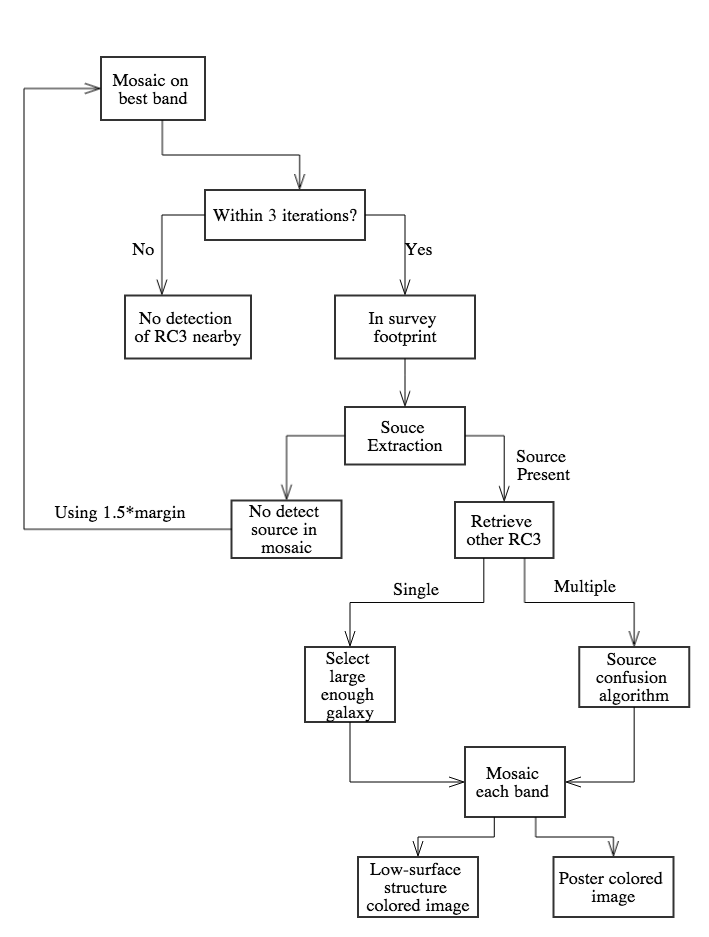
\includegraphics[width=0.5\textwidth]{figures/algorithm.png}
\caption{ A flowchart detailing the basic steps employed by our pipeline to first construct calibrated FITS image mosaics for each photometric band in an imaging survey of the target galaxy, followed by the construction of color-composite images for the target galaxy.}
\label{flowchart}
\end{figure}

\subsection{Algorithm Enhancements}

The montage software can be accessed via the Virtual Astrophysical Observatory (VAO) Image Mosaic Service at the Infrared Science Archive (IRSA) website to robustly generate mosaic images from multiple surveys, including from both the SDSS and DSS. Given the nature of the RC3 catalog, however, we had to overcome two challenges when including montage as part of our overall mosaicking pipeline. First, the relatively large positional uncertainty present for some galaxies within the RC3 catalog meant a mosaic could be automatically generated by using montage that either had the target galaxy off-center, or worse entirely missing from the mosaic. Second, since galaxies are often in groups or clusters, a positional uncertainty can lead to a mis-identification of the target galaxy within the constructed mosaic. As a result, two components are developed within our pipeline to address these two issues in order to generate a mosaic image centered on the appropriate galaxy.

\subsubsection{Positional Update\label{pos-sec}} 

We created a class, called $\texttt{RC3}$, to encapsulate the data and methods relevant to the RC3 sources. Each $\texttt{RC3}$ instance contains the catalog RC3 coordinate information, any updated coordinate information, radius, and a unique identifier. While we could have adopted a standard numerical identifier scheme, we instead chose to adopt each galaxy's Catalogue of Principal Galaxies (PGC) number, since this is a unique identifier for each RC3 galaxy that is also already present in the original RC3 catalog. This unique name provides unambiguity for our pipeline, and is also used for naming the generated data products and serving these same products via our website.

To overcome the problem of inaccurate positions discussed in \S\ref{sec:position}, we developed an approach that finds the target galaxy in the imaging data and uses this position to update the astrometric information appropriately. This algorithm is implemented in the $\texttt{source\_info}$ method of the $\texttt{RC3}$ class, and first generates a mosaic with a field of view roughly six times larger than the radius of the target galaxy.  Next, SExtractor is used to detect all sources on the newly generated mosaic. The selected mosaic size is generally sufficient to ensure that will be able to determine an accurate background sky level. Of all detected sources, only those with a radius greater than 5.94 arcseconds are retained. This size was empirically selected to eliminate most stellar sources and background noise spikes while still retaining the subset of RC2 galaxies contained in the RC3 catalog that are smaller than one arcminute as described by~\citealp{rc2}. 

At this point, our pipeline is in one of three states depending on whether there are zero, one, or more galaxies detected by SExtractor on the new mosaic that might be RC3 galaxies. First, if there are zero candidate RC3 galaxies in the new mosaic, we recursively create larger mosaics until either an RC3 candidate galaxy is detected or we complete three iterations. If only one candidate galaxy is detected, the pipeline proceeds directly to the color image generation step. If multiple large galaxies are detected, the pipeline completes the source confusion process outlined in \S\ref{sec:sc}. At the end of this process, we will have generated mosaic images in all five bands as long as at least one candidate RC3 galaxy was detected.

Once the mosaic images have been constructed in all bands for the given survey, we select images observed through three different filters and recombine them into a color mosaic image by using STIFF\label{sec:best_low}. The three bands selected are the $g$, $r$, and $i$ bands for the SDSS, which has five bands, and the $B_J$, $R_F$, and $I_N$ bands for the DSS survey, which only has these three bands. At this point, two color images are generated (although this number can be altered if necessary). The first color image generated emphasize low surface brightness structures, such as the halo around a galaxy, or interaction tidal streams. The second color image generated is a poster or publication quality image that uses higher background cuts to ensure a clean, highly contrasted image. We note that to construct a color image, our pipeline does require at least three bands. Fortunately, most photometric surveys meet this criterion, which is not surprising since the construction of a color-color plot, which are used to minimize the effects of extinction and identify stellar or extragalactic source populations, require at least three bands~\citep[see, e.g.,][]{2mass}.

\subsubsection{Source Confusion\label{sec:sc}}

\begin{figure}
\centering
  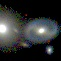
\includegraphics[width=.225\textwidth]{figures/PGC58b4SC}
  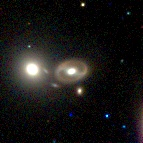
\includegraphics[width=.225\textwidth]{figures/PGC58afterSC}
\caption{ A visual demonstration, using SDSS image data, of our source confusion algorithm, see Figure~\ref{fig:positional_update_plot} for a wider angle view of this same field. (Left) A color-composite image made from mosaicked $g$, $r$, and $i$ FITS images. (Right) The regenerated color-composite image made from the original data after the source confusion algorithm has been applied, resulting in a recentering on the target galaxy PGC58.}
\label{fig:SCdemo}
\end{figure}

The second challenge our pipeline was forced to tackle was the source confusion problem. Since large galaxies are often physically located near other galaxies, any astrometric error in the location of our target RC3 galaxy could result in source confusion on a generated mosaic (see Figure~\ref{fig:positional_update_plot} for a visual demonstration). To tackle this challenge, we first assumed that any galaxy large enough to cause confusion would also be present in the original RC3 catalog. This assumption is supported by the fact that the RC3 catalog is reasonably complete for galaxies with apparent diameters larger than one arcminute. 

The algorithm we developed to overcome this challenge first identifies all RC3 galaxies that may lie within the newly generated mosaic image, and second matches this list to the list of galaxies that were actually detected by SExtractor within the mosaic image. The list of RC3 galaxies is generated by the $\texttt{otherRC3}$ method that is part of the $\texttt{Server}$ class described in \S~\ref{sec:server}. By default, this method queries the VizieR Catalog to obtain this information. Alternatively, this method can be overridden if a survey provides this information directly, like the SDSS, which contains an RC3 table in its SkyServer database. 

\begin{figure}[h]
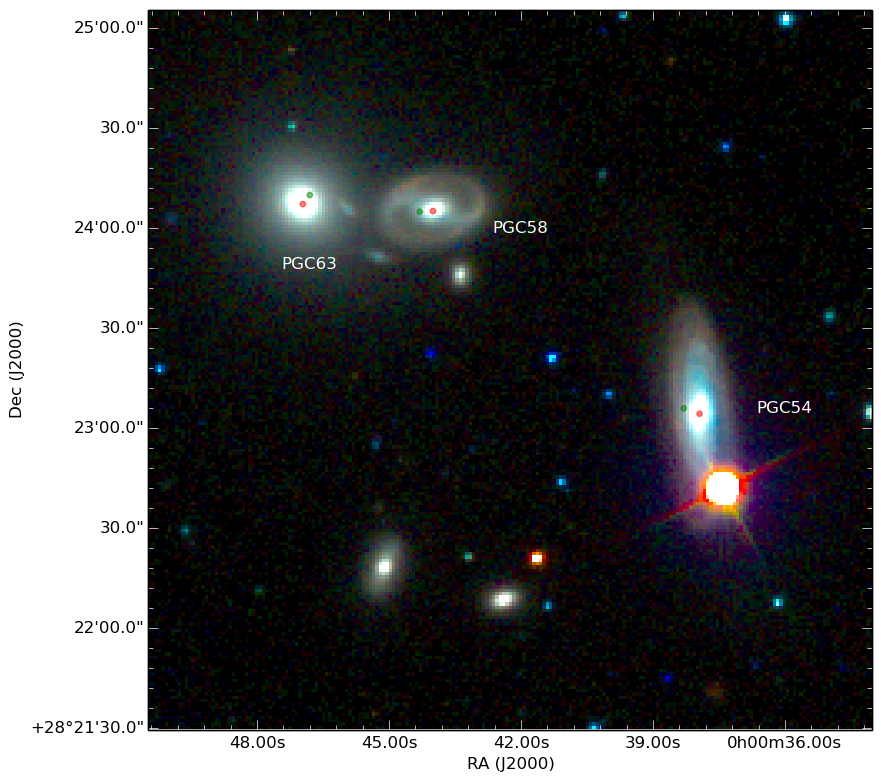
\includegraphics[width=0.5\textwidth]{figures/navigator}
\caption{A visual demonstration of the results of the source confusion algorithm for three RC3 Galaxies showing the original RC3 catalog galaxy coordinates (green markers) and our newly calculated coordinates (red markers).}
\label{fig:positional_update_plot}
\end{figure}

Naively, this cross-match process might appear to be simple; however, since each of these RC3 galaxies may have inaccurate astrometry, the problem becomes non-trivial. To tackle this challenge, we make the reasonable assumption that any positional inaccuracies are due to instrumental or measurement errors that might affect a galaxy's absolute position but not the relative positions of each galaxy. Thus we identify the \textit{n} RC3 galaxies that potentially lie within the mosaic image from VizieR, and compute all possible relative positional differences between these candidate galaxies. Next, we compare this list with the positional differences computed between the galaxies detected in the actual image by SExtractor. From this list of cross-matched differences, we identify each RC3 galaxy in the image, correct the overall astrometry for each detected RC3 galaxy, and regenerate a new mosaic centered on the correct location). We have verified the accuracy of these assumptions by using the SDSS, where find a success rate of 99.97\%. Furthermore, we have found that this approach correctly resolves up to five RC3 sources in a single mosaic.
	
\subsection{Pipeline}

To simplify the application of our approach to other catalogs and/or surveys, we developed an automated pipeline to generate the FITS image mosaics and color-composite images. This pipeline is built by using classes that encapsulate specific data that might be relative to a certain catalog, like the RC3, or to a particular survey, like the SDSS. The overall class relationship is presented in Figure~\ref{fig:hierarchy}, which highlights three abstract classes: $\texttt{Survey}$, $\texttt{Catalog}$, and $\texttt{Server}$, which simplify the incorporation of new catalog data or surveys into our pipeline. In the following subsections, we discuss several of these classes in more detail.

\begin{figure}[h]
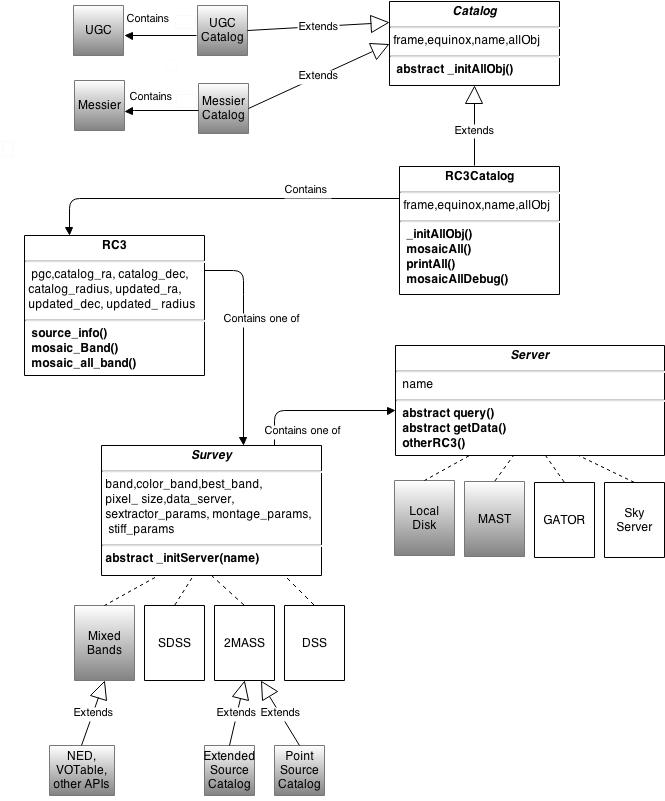
\includegraphics[width=0.5\textwidth]{figures/hierarchy}
\caption{A unified modeling language (UML) class diagram showing the relationships between different classes in the mosaicking pipeline. Grey-filled boxes shows possible extensions of this pipeline.
\label{fig:hierarchy}
}
\end{figure}

\subsubsection{Server\label{sec:server}}

The primary abstract class used by the pipeline is the $\texttt{Server}$ class, which encapsulates the two main tasks of data acquisition: querying imaging data and retrieving the imaging data from the actual server. Many recent surveys provide an application programming interface (API) that enables data access either by using SQL or a customized query mechanism. To actually implement a subclass of the $\texttt{Server}$ class, a mapping between the positional values of galaxies in a particular catalog and the recorded image data for the particular survey must be established. For example, SDSS image frames are uniquely identified by a particular combination of \textit{run}, \textit{camcol}, and \textit{field}, while 2MASS identifies images with a sexagesimal, equatorial position-based source name. For those surveys where this type of mapping has not already been established, such as the imaging data from the POSS-II survey, a subclass can establish a new naming scheme.

In addition to these primary tasks, each $\texttt{Server}$ subclass also must implement functionality to build and execute queries as required by the montage mosaic software. By using a $\texttt{Server}$ class as opposed to a $\texttt{DataObject}$ class enables code reusability across various surveys that can be accessed via common server tools. For example, this approach allows the pipeline to easily use the IRSA GATOR query service~\citep{irsa} and Astroquery\footnote{\url{http://astroquery.readthedocs.org/}}.

\subsubsection{Catalog Objects}

The current version of the pipeline, which solely generates mosaic images of RC3 galaxies, does not contain an abstract $\texttt{CatalogObject}$ class. As a future extension, this would be a beneficial addition as it would be helpful to have a generic class that provides a similar functionality as the $\texttt{RC3Objects}$ class. These functions contain basic information about the particular object and are survey-independent. They also perform the essential mosaicking features on a per-object basis. Therefore, these functions not only can be used for comparing resulting mosaics from multiple surveys (see, e.g., \S\ref{fig:comparison}), but these methods can also be conveniently used within the $\texttt{Catalog}$ class. 

The final step in the mosaic procedure generates two TIFF color images as described in \S\ref{sec:best_low}.  When extending the pipeline to other surveys, prototyping work should be done to determine the optimal STIFF parameters in order to generate color-composite images that best capture the details in the telescope-specific imaging by following the guidelines in \citet{stiff}.

\subsubsection{Catalog}

The simplest abstract class contained in the pipeline is the $\texttt{Catalog}$ class, which simply contains a list of objects in a particular catalog. While the use of such an abstract container class might seem superfluous, by using this class, the pipeline is able to cleanly separate the basic mosaic functionality for individual galaxies from the functionality required for an entire catalog. This capability enables a direct study of a single object, enables a processing of all sources listed in the derived $\texttt{Catalog}$ class, or simplifies the debugging process. By using this abstract barrier, we ensure minimal changes are required in the class structure if the pipeline is modified to support imaging data from a new survey.

\section{Results\label{results-sec}}

\begin{figure}[h]
\centering
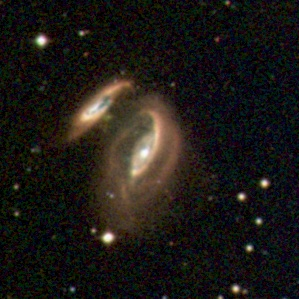
\includegraphics[width=0.4\textwidth]{figures/DSS_120_BEST}
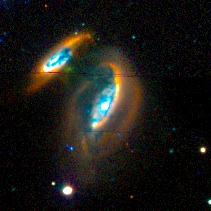
\includegraphics[width=0.4\textwidth]{figures/SDSS_120_LOW}	
\caption{PGC120 mosaic from POSS-II (top) and SDSS (bottom). The two images are of different scale.}
\label{fig:comparison}
\end{figure}

\begin{figure}[h]
\centering
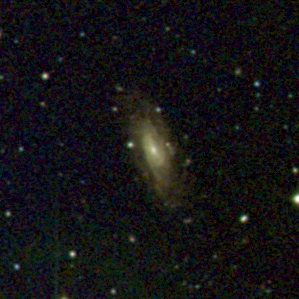
\includegraphics[width=0.4\textwidth]{figures/DSS_1154_BEST}	
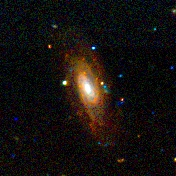
\includegraphics[width=0.4\textwidth]{figures/SDSS_1154_BEST}
\caption{PGC1746 mosaic from POSS-II (top) and SDSS (bottom). The two images are of different scale.}
\label{sdss_dss_comp}
\end{figure}

\subsection{Mosaicking Results}

Of the total 23,011 galaxies described in the RC3 catalog, 12,418 lie within the SDSS DR10 footprint. Our automated pipeline successfully generated mosaics for 76.58\% of these galaxies. Of these, 4,283 RC3 galaxies were mosaicked by using an updated position that was more than one arcminute away from the recorded RC3 astrometric position. On an 8-core linux server, the pipeline averaged 80 RC3 galaxy mosaics per hour for the SDSS data, which was retrieved from a remote SDSS data repository. The final data products, the five band FITS mosaic images and two color composite images for each galaxy, occupy approximately twenty GBs.

The POSS-II data has full sky coverage, thus all 23,011 RC3 galaxies are covered by the POSS-II footprint. Of this full sample, the automated pipeline was successful for all RC3 galaxies, except for 8,431 galaxies that produced a STIFF error (see \S~\ref{error} for a discussion of this condition). For the POSS-II mosaics, 3,431 RC3 galaxies were mosaicked by using an updated position that was more than one arcminute away from the recorded RC3 astrometric position. Given the larger base images for the POSS-II survey ($\sim1.1$ GB each), it is not surpassing that our pipeline was slower when creating POSS-II mosaics, averaging about fifty galaxies per hour on the same machine used for the SDSS mosaicking. The finished data products for the POSS-II sample of galaxies occupies approximately 10 GBs.

\subsection{Pipeline Performance}	

The majority of the processing time for our pipeline is in transferring the raw FITS image data from the survey data site to the processing site. However, we have explored techniques to improve the overall performance of the pipeline. First, we accelerate the mosaicking process by performing the positional update on only a single band from the bands available from a given survey. The target band is designated as the $\texttt{best\_band}$, and given the results from this single band, the other image FITs mosaics are performed only once per object. For example, for the SDSS we use r-band images, since the r-band filter since transmission has the highest quantum efficiency~\citep{edr}.

Since data transfer dominates the overall processing time, we do not employ traditional parallel programming techniques (we could, however, employ embarrassingly parallel techniques since mosaic images are constructed independently). Thus, even though Montage's modular design enables its performance to scale with the number of processors~\citep{montage}, our pipeline would not be accelerated by using  Message Passing Interface (MPI).  Other factors that affect the runtime include the sky coverage of a particular survey and the response speed of query from a survey archive.

One technique that could be employed to accelerate our pipeline would be local image caching, or alternatively the capability of executing our pipeline within a survey archive. We have designed our pipeline by using a class hierarchy that enables subclassing of the $\texttt{Server}$ class to specify the location of a survey's raw FITS images. However, downloading an entire survey's imaging data set for this purpose is unlikely to be beneficial (if done solely for this task), since that would likely take significantly more time than simply downloading the required input raw FITs imaged required for the mosaics when running the pipeline.

\subsection{Technical Details}

Due to the recent rise in the popularity of the Python programming language, we developed our pipeline by using Python 2.7.6. As a result, our pipeline's dependencies are widely supported, which simplifies the extension of our work to future datasets. The majority of the mosaicking actions are done by calls to the Montage API along with the AstroPy Montage wrapper\footnote{\url{http://www.astropy.org/montage-wrapper/}} developed by~\cite{montpy}. The final color-composite images are generated by using Astromatic's STIFF v.2.4~\citep{stiff}. 

Our combination of these two programs allows us to make use of their best features. Montage excels at creating scientifically-calibrated images that retains the astrometry and photometry of input sources during the image reprojection. Our choice was also aided by the fact that the efficacy of montage was already demonstrated by the montage developers by using SDSS and POSS-II image data sets~\citep{montage}. On the other hand, STIFF provides the flexibility of adjusting a number of parameters to optimize the appearance of the final color-composite image, and also automatically estimates the upper and lower limits for the dynamic range of the final color image by using statistics derived from a pixel histogram. 

Other major steps in our pipeline that required custom code development include query construction, query result processing, source extraction on the mosaicked image, and the development of a web-accessible database to facilitate access to our data products. We use the SDSS Command line query tool written by~\cite{sqlclref}  to submit SQL queries to SkyServer and we use Astroquery as a more general archive query tool and to find other RC3 galaxies that lie within a field by using the VizieR catalog database. For IRSA and most web databases, querying consists of building a URL string, submitting the query, and parsing the resulting  raw text or XML file returned by \texttt{wget}. Source extraction was performed by using SExtractor v.2.19.5~\citep{sextractor} with standard processing parameters. Our web-accessible database was created by using the Python sqlite3 module, and the web search interface was written in PHP with interacting HTML elements.

\subsection{Known Error Conditions \label{error}}

As a good programming practice, we included a series of exception handling and error prevention mechanisms throughout our pipeline. However, the actual running of our pipeline on a survey still results in occasional errors. To indicate a non-successful operation of our pipeline for a particular source, we developed several error flags that are encoded in our web-accessible database for each survey.


\begin{verbatim}
Error Information
0 = no error
1 = mosaicAll error
2 = stiff error 
3 = strange error
4 = Montage image reprojection failure
5 = mSubImage failure
\end{verbatim}

In the rest of this section, we detail the processing conditions that can generate the corresponding error condition.
\begin{enumerate}

\item  \texttt{mosaicAll} error is a general error that is raised when the pipeline fails to generate mosaics in all bands.

\item  STIFF enforces that the mosaic FITS used for RGB mapping but must all have exactly the same dimensions in order to generate a color-composite image. On occasion, a color-composite image fails to be produced because at least one image is not of the same size as the other two.  For the SDSS this seems to happen predominantly in the $g$-band, and this also happens more frequently for the POSS-II data.

\item  In the source confusion algorithm, we query the VizieR catalog to identify all galaxies that pass a size cut inside a search radius. This is done by using the PGC name as a key and the positions as the values. If no galaxies are returned by this search, the pipeline raises this error condition.

\item  $\texttt{mProjectExec}$ is the Montage procedure that creates the reprojected image from the original FITS files. Sometimes reprojected images are not created, even when the Montage processes complete successfully and the  debug statements clearly state that the reprojection was successful. In this case, the reprojection table and header files are corrupted, which will produce an error condition in the subsequent mosaicking steps. To prevent a complete failure, we have implemented an error prevention mechanism to ensure that the mosaic generation procedures terminate correctly for these cases, and we denote the problematic galaxy as a \texttt{failed\_projection}, which can be examined manually offline. 


\item $\texttt{mSubImage}$ crops a finished mosaic to the specified final size. In some cases, the desired final image (e.g., the poster image size) exceeds the actual size of the generated mosaic image. This can arise if a target RC3 galaxy lies near the edge of a survey's observed footprint or the survey has missing or masked data near the target galaxy. In these cases, Montage throws an error indicating that a new image could not be made by cropping the existing image. To circumvent this error condition, we set the field size to be twice the margin, where we define the margin as the distance from the center of the galaxy to the edge of the mosaic image. The margin value is dynamically updated by the recursive algorithm as necessary. Since we are cropping to a square image, the margin should thus be one-half of the final FITS image size after the cropping process completes. If the double-margin crop fails, we attempt a smaller field size of one margin. If this second attempt also fails, we record this error condition and proceed onto the next galaxy. 

\end{enumerate}	 

 \section{Conclusion\label{conc-sec}}
 
Wide-area sky surveys are used, by design, to answer fundamental questions regarding the formation and evolution of large-scale structure and of the cosmological history of the universe. But these data can be used for many other purposes. The mosaicking pipeline described in this paper, for example, provides a convenient way to generate mosaic images for specific sources from an archived set of sky survey images.  Furthermore, this pipeline can be easily be adapted to work with future data to create scientifically-calibrated FITS mosaics as well as color-composite images. The source code and documentation for the pipeline described in this paper can be found in the project repository\footnote{\url{http://github.com/ProfessorBrunner/rc3-pipeline/}}. In addition, we have provided documentation on GitHub that will guide other investigators to adapt the pipeline for alternative imaging data sets.

To ensure that the generated mosaic images are centered on the target source, we implemented an algorithm that automatically determines the correct source astrometry, updates the source catalog appropriately, and generates mosaic images centered on the newly updated coordinate location. Finally, to demonstrate the efficacy of this new pipeline, we generated FITS image mosaics and color-composite images of galaxies in the RC3 catalog by using the SDSS and POSS-II data. All of these data products are publicly released and accessible via a searchable web form on the Laboratory for Cosmological Data Mining website\footnote{\url{http://lcdm.astro.illinois.edu/data/rc3/}}.

By developing this new pipeline, we can generate image mosaics using newly-obtained data, which will enable a more complete sky coverage for a given source catalog or the construction of potentially higher resolution images or images in other wavelengths. In addition, the pipeline simplifies the extension of this work to either user-defined catalogs or to other published catalogs, such as the Messier Catalog or the New General Catalog. Furthermore, a specific scientific inquiry may require the construction of a user-defined catalog  by imposing selection criteria to study certain types of objects. To accomplish this task, a user simply needs to generate a text file containing source positions, source radii, and unique identifier for each source, which can subsequently be used as input to the pipeline. 

The scientifically calibrated FITS image mosaics generated by the pipeline for a specific galaxy catalog can be used both for individual source studies, as well as ensemble studies of source populations. In addition, the multi-band FITS mosaic images can be combined with calibrated mosaic images at different wavelengths into new, multi-band color images by using mosaic images from other surveys. This can be especially beneficial when a survey has only one or two bands, such as the POSS-I~\citep{poss1} or GALEX~\citep{galex}, as long as the image sizes are adjusted to match. The generated FITS mosaic images can also be used as inputs to
existing tools such as Astrometry.net~\citep{astrometry.net} or SExtractor~\citep{sextractor} for subsequent processing or to tools like ds9~\citep{ds9}, Alladin~\citep{aladin}, or APLpy~\citep{aplpy} for scientific visualization.

Finally, the SDSS and POSS-II mosaic images that we have generated and publicly released via the LCDM website may prove be useful during the commissioning and data management processing of new surveys such as the DES or LSST. With the growth in the size of  imaging cameras on new and existing telescopes, large, nearby galaxies, such as those in the RC3 catalog, need to be properly identified and possibly masked in order to minimize the loss of imaging details from saturated CCDs. The updated RC3 coordinates indicate regions of the sky that may be affected by these large galaxies, and the FITS mosaic images can be used to model-fit the galaxy's shape and light distribution. Alternatively, this same information can be used to place spectroscopic fibers on RC3 catalog sources. 

\section*{Acknowledgements}
\footnotesize

The work was supported by the Google Summer of Code Program. RJB would also like to acknowledge support from the National Science Foundation Grant No. AST-1313415. We thank Harold G. Corwin Jr. for helpful discussion that helped this work. 

This research made use of Montage, funded by the National Aeronautics and Space Administration's Earth Science Technology Office, Computation Technologies Project, under Cooperative Agreement Number NCC5-626 between NASA and the California Institute of Technology. Montage is maintained by the NASA/IPAC Infrared Science Archive. This research made use of Astropy, a community-developed core Python package for Astronomy~\citep{astropy}.

Funding for SDSS-III has been provided by the Alfred P. Sloan Foundation, the Participating Institutions, the National Science Foundation, and the U.S. Department of Energy Office of Science. The SDSS-III web site is http://www.sdss3.org/. SDSS-III is managed by the Astrophysical Research Consortium for the Participating Institutions of the SDSS-III Collaboration including the University of Arizona, the Brazilian Participation Group, Brookhaven National Laboratory, University of Cambridge, Carnegie Mellon University, University of Florida, the French Participation Group, the German Participation Group, Harvard University, the Instituto de Astrofisica de Canarias, the Michigan State/Notre Dame/JINA Participation Group, Johns Hopkins University, Lawrence Berkeley National Laboratory, Max Planck Institute for Astrophysics, Max Planck Institute for Extraterrestrial Physics, New Mexico State University, New York University, Ohio State University, Pennsylvania State University, University of Portsmouth, Princeton University, the Spanish Participation Group, University of Tokyo, University of Utah, Vanderbilt University, University of Virginia, University of Washington, and Yale University

\bibliography{rc3_pipeline}
\bibliographystyle{elsarticle-harv}

\end{document}
